%%%%%%%%%%%%%%%%%%%%%%%%%%%%%%%%%%%%%%%%%
% Style based on: The Legrand Orange Book - Version 1.4 (12/4/14)
%
% The original template has been downloaded from:
% http://www.LaTeXTemplates.com
%
% Original author:
% Mathias Legrand (legrand.mathias@gmail.com)
%
% License:
% CC BY-NC-SA 3.0 (http://creativecommons.org/licenses/by-nc-sa/3.0/)
%%%%%%%%%%%%%%%%%%%%%%%%%%%%%%%%%%%%%%%%%

%----------------------------------------------------------------------------------------
%	PACKAGES AND OTHER DOCUMENT CONFIGURATIONS
%----------------------------------------------------------------------------------------

\documentclass[11pt,fleqn,oneside,openany]{book} % Default font size and left-justified equations

\usepackage[top=3cm,bottom=3cm,left=3.2cm,right=3.2cm,headsep=10pt,a4paper]{geometry} % Page margins

\usepackage{xcolor} % Required for specifying colors by name
\definecolor{ocre}{RGB}{243,102,25} % Define the orange color used for highlighting throughout the book
\definecolor{brown}{RGB}{192,81,20} % Define the brown color used for highlighting of URLs throughout the book

% Font Settings
\usepackage{avant} % Use the Avantgarde font for headings
%\usepackage{times} % Use the Times font for headings
\usepackage{mathptmx} % Use the Adobe Times Roman as the default text font together with math symbols from the Sym­bol, Chancery and Com­puter Modern fonts

\usepackage{microtype} % Slightly tweak font spacing for aesthetics
\usepackage[utf8]{inputenc} % Required for including letters with accents
\usepackage[T1]{fontenc} % Use 8-bit encoding that has 256 glyphs

% Bibliography
%\usepackage[style=alphabetic,sorting=nyt,sortcites=true,autopunct=true,babel=hyphen,hyperref=true,abbreviate=false,backref=true,backend=biber]{biblatex}
%\addbibresource{bibliography.bib} % BibTeX bibliography file
%\defbibheading{bibempty}{}

% Index
%\usepackage{calc} % For simpler calculation - used for spacing the index letter headings correctly
%\usepackage{makeidx} % Required to make an index
%\makeindex % Tells LaTeX to create the files required for indexing

%----------------------------------------------------------------------------------------
%	VARIOUS REQUIRED PACKAGES
%----------------------------------------------------------------------------------------

\usepackage{titlesec} % Allows customization of titles

\usepackage{graphicx} % Required for including images
\graphicspath{{images/}} % Specifies the directory where images are stored

\usepackage{lipsum} % Inserts dummy text

\usepackage{tikz} % Required for drawing custom shapes

\usepackage[english]{babel} % English language/hyphenation

\usepackage{enumitem} % Customize lists
\setlist{nolistsep} % Reduce spacing between bullet points and numbered lists

\usepackage{booktabs} % Required for nicer horizontal rules in tables

\usepackage{eso-pic} % Required for specifying an image background in the title page

%----------------------------------------------------------------------------------------
%	MAIN TABLE OF CONTENTS
%----------------------------------------------------------------------------------------

\usepackage{titletoc} % Required for manipulating the table of contents

\contentsmargin{0cm} % Removes the default margin
% Chapter text styling
\titlecontents{chapter}[1.25cm] % Indentation
{\addvspace{15pt}\large\sffamily\bfseries} % Spacing and font options for chapters
{\color{ocre!60}\contentslabel[\Large\thecontentslabel]{1.25cm}\color{ocre}} % Chapter number
{}  
{\color{ocre!60}\normalsize\sffamily\bfseries\;\titlerule*[.5pc]{.}\;\thecontentspage} % Page number
% Section text styling
\titlecontents{section}[1.25cm] % Indentation
{\addvspace{5pt}\sffamily\bfseries} % Spacing and font options for sections
{\contentslabel[\thecontentslabel]{1.25cm}} % Section number
{}
{\sffamily\hfill\color{black}\thecontentspage} % Page number
[]
% Subsection text styling
\titlecontents{subsection}[1.25cm] % Indentation
{\addvspace{1pt}\sffamily\small} % Spacing and font options for subsections
{\contentslabel[\thecontentslabel]{1.25cm}} % Subsection number
{}
{\sffamily\;\titlerule*[.5pc]{.}\;\thecontentspage} % Page number
[] 

%----------------------------------------------------------------------------------------
%	MINI TABLE OF CONTENTS IN CHAPTER HEADS
%----------------------------------------------------------------------------------------

% Section text styling
\titlecontents{lsection}[0em] % Indendating
{\footnotesize\sffamily} % Font settings
{}
{}
{}

% Subsection text styling
\titlecontents{lsubsection}[.5em] % Indentation
{\normalfont\footnotesize\sffamily} % Font settings
{}
{}
{}
 
%----------------------------------------------------------------------------------------
%	PAGE HEADERS
%----------------------------------------------------------------------------------------

\usepackage{fancyhdr} % Required for header and footer configuration

\pagestyle{fancy}
\renewcommand{\chaptermark}[1]{\markboth{\sffamily\normalsize\bfseries\chaptername\ \thechapter.\ #1}{}} % Chapter text font settings
\renewcommand{\sectionmark}[1]{\markright{\sffamily\normalsize\thesection\hspace{5pt}#1}{}} % Section text font settings
\fancyhf{} \fancyhead[LE,RO]{\sffamily\normalsize\thepage} % Font setting for the page number in the header
\fancyhead[LO]{\rightmark} % Print the nearest section name on the left side of odd pages
\fancyhead[RE]{\leftmark} % Print the current chapter name on the right side of even pages
\renewcommand{\headrulewidth}{0.5pt} % Width of the rule under the header
\addtolength{\headheight}{2.5pt} % Increase the spacing around the header slightly
\renewcommand{\footrulewidth}{0pt} % Removes the rule in the footer
\fancypagestyle{plain}{\fancyhead{}\renewcommand{\headrulewidth}{0pt}} % Style for when a plain pagestyle is specified

% Removes the header from odd empty pages at the end of chapters
\makeatletter
\renewcommand{\cleardoublepage}{
\clearpage\ifodd\c@page\else
\hbox{}
\vspace*{\fill}
\thispagestyle{empty}
\newpage
\fi}

%----------------------------------------------------------------------------------------
%	THEOREM STYLES
%----------------------------------------------------------------------------------------

\usepackage{amsmath,amsfonts,amssymb,amsthm} % For math equations, theorems, symbols, etc

\newcommand{\intoo}[2]{\mathopen{]}#1\,;#2\mathclose{[}}
\newcommand{\ud}{\mathop{\mathrm{{}d}}\mathopen{}}
\newcommand{\intff}[2]{\mathopen{[}#1\,;#2\mathclose{]}}
\newtheorem{notation}{Notation}[chapter]

%%%%%%%%%%%%%%%%%%%%%%%%%%%%%%%%%%%%%%%%%%%%%%%%%%%%%%%%%%%%%%%%%%%%%%%%%%%
%%%%%%%%%%%%%%%%%%%% dedicated to boxed/framed environements %%%%%%%%%%%%%%
%%%%%%%%%%%%%%%%%%%%%%%%%%%%%%%%%%%%%%%%%%%%%%%%%%%%%%%%%%%%%%%%%%%%%%%%%%%
\newtheoremstyle{ocrenumbox}% % Theorem style name
{0pt}% Space above
{0pt}% Space below
{\normalfont}% % Body font
{}% Indent amount
{\small\bf\sffamily\color{ocre}}% % Theorem head font
{\;}% Punctuation after theorem head
{0.25em}% Space after theorem head
{\small\sffamily\color{ocre}\thmname{#1}\nobreakspace\thmnumber{\@ifnotempty{#1}{}\@upn{#2}}% Theorem text (e.g. Theorem 2.1)
\thmnote{\nobreakspace\the\thm@notefont\sffamily\bfseries\color{black}---\nobreakspace#3.}} % Optional theorem note
\renewcommand{\qedsymbol}{$\blacksquare$}% Optional qed square

\newtheoremstyle{blacknumex}% Theorem style name
{5pt}% Space above
{5pt}% Space below
{\normalfont}% Body font
{} % Indent amount
{\small\bf\sffamily}% Theorem head font
{\;}% Punctuation after theorem head
{0.25em}% Space after theorem head
{\small\sffamily{\tiny\ensuremath{\blacksquare}}\nobreakspace\thmname{#1}\nobreakspace\thmnumber{\@ifnotempty{#1}{}\@upn{#2}}% Theorem text (e.g. Theorem 2.1)
\thmnote{\nobreakspace\the\thm@notefont\sffamily\bfseries---\nobreakspace#3.}}% Optional theorem note

\newtheoremstyle{blacknumbox} % Theorem style name
{0pt}% Space above
{0pt}% Space below
{\normalfont}% Body font
{}% Indent amount
{\small\bf\sffamily}% Theorem head font
{\;}% Punctuation after theorem head
{0.25em}% Space after theorem head
{\small\sffamily\thmname{#1}\nobreakspace\thmnumber{\@ifnotempty{#1}{}\@upn{#2}}% Theorem text (e.g. Theorem 2.1)
\thmnote{\nobreakspace\the\thm@notefont\sffamily\bfseries---\nobreakspace#3.}}% Optional theorem note

%%%%%%%%%%%%%%%%%%%%%%%%%%%%%%%%%%%%%%%%%%%%%%%%%%%%%%%%%%%%%%%%%%%%%%%%%%%
%%%%%%%%%%%%% dedicated to non-boxed/non-framed environements %%%%%%%%%%%%%
%%%%%%%%%%%%%%%%%%%%%%%%%%%%%%%%%%%%%%%%%%%%%%%%%%%%%%%%%%%%%%%%%%%%%%%%%%%
\newtheoremstyle{ocrenum}% % Theorem style name
{5pt}% Space above
{5pt}% Space below
{\normalfont}% % Body font
{}% Indent amount
{\small\bf\sffamily\color{ocre}}% % Theorem head font
{\;}% Punctuation after theorem head
{0.25em}% Space after theorem head
{\small\sffamily\color{ocre}\thmname{#1}\nobreakspace\thmnumber{\@ifnotempty{#1}{}\@upn{#2}}% Theorem text (e.g. Theorem 2.1)
\thmnote{\nobreakspace\the\thm@notefont\sffamily\bfseries\color{black}---\nobreakspace#3.}} % Optional theorem note
\renewcommand{\qedsymbol}{$\blacksquare$}% Optional qed square
\makeatother

% Defines the theorem text style for each type of theorem to one of the three styles above
\newcounter{dummy} 
\numberwithin{dummy}{section}
\theoremstyle{ocrenumbox}
\newtheorem{theoremeT}[dummy]{Theorem}
\newtheorem{problem}{Problem}[chapter]
\newtheorem{exerciseT}{Exercise}[chapter]
\theoremstyle{blacknumex}
\newtheorem{exampleT}{Example}[chapter]
\theoremstyle{blacknumbox}
\newtheorem{vocabulary}{Vocabulary}[chapter]
\newtheorem{definitionT}{Definition}[section]
\newtheorem{corollaryT}[dummy]{Corollary}
\theoremstyle{ocrenum}
\newtheorem{proposition}[dummy]{Proposition}

%----------------------------------------------------------------------------------------
%	DEFINITION OF COLORED BOXES
%----------------------------------------------------------------------------------------

\RequirePackage[framemethod=default]{mdframed} % Required for creating the theorem, definition, exercise and corollary boxes

% Theorem box
\newmdenv[skipabove=7pt,
skipbelow=7pt,
backgroundcolor=black!5,
linecolor=ocre,
innerleftmargin=5pt,
innerrightmargin=5pt,
innertopmargin=5pt,
leftmargin=0cm,
rightmargin=0cm,
innerbottommargin=5pt]{tBox}

% Exercise box	  
\newmdenv[skipabove=7pt,
skipbelow=7pt,
rightline=false,
leftline=true,
topline=false,
bottomline=false,
backgroundcolor=ocre!10,
linecolor=ocre,
innerleftmargin=5pt,
innerrightmargin=5pt,
innertopmargin=5pt,
innerbottommargin=5pt,
leftmargin=0cm,
rightmargin=0cm,
linewidth=4pt]{eBox}	

% Definition box
\newmdenv[skipabove=7pt,
skipbelow=7pt,
rightline=false,
leftline=true,
topline=false,
bottomline=false,
linecolor=ocre,
innerleftmargin=5pt,
innerrightmargin=5pt,
innertopmargin=0pt,
leftmargin=0cm,
rightmargin=0cm,
linewidth=4pt,
innerbottommargin=0pt]{dBox}	

% Corollary box
\newmdenv[skipabove=7pt,
skipbelow=7pt,
rightline=false,
leftline=true,
topline=false,
bottomline=false,
linecolor=gray,
backgroundcolor=black!5,
innerleftmargin=5pt,
innerrightmargin=5pt,
innertopmargin=5pt,
leftmargin=0cm,
rightmargin=0cm,
linewidth=4pt,
innerbottommargin=5pt]{cBox}

% Creates an environment for each type of theorem and assigns it a theorem text style from the "Theorem Styles" section above and a colored box from above
\newenvironment{theorem}{\begin{tBox}\begin{theoremeT}}{\end{theoremeT}\end{tBox}}
\newenvironment{exercise}{\begin{eBox}\begin{exerciseT}}{\hfill{\color{ocre}\tiny\ensuremath{\blacksquare}}\end{exerciseT}\end{eBox}}
\newenvironment{definition}{\begin{dBox}\begin{definitionT}}{\end{definitionT}\end{dBox}}	
\newenvironment{example}{\begin{exampleT}}{\hfill{\tiny\ensuremath{\blacksquare}}\end{exampleT}}		
\newenvironment{corollary}{\begin{cBox}\begin{corollaryT}}{\end{corollaryT}\end{cBox}}	

%----------------------------------------------------------------------------------------
%	REMARK ENVIRONMENT
%----------------------------------------------------------------------------------------

\newenvironment{remark}{\par\vspace{10pt}\small % Vertical white space above the remark and smaller font size
\begin{list}{}{
\leftmargin=35pt % Indentation on the left
\rightmargin=25pt}\item\ignorespaces % Indentation on the right
\makebox[-2.5pt]{\begin{tikzpicture}[overlay]
\node[draw=ocre!60,line width=1pt,circle,fill=ocre!25,font=\sffamily\bfseries,inner sep=2pt,outer sep=0pt] at (-15pt,0pt){\textcolor{ocre}{R}};\end{tikzpicture}} % Orange R in a circle
\advance\baselineskip -1pt}{\end{list}\vskip5pt} % Tighter line spacing and white space after remark

%----------------------------------------------------------------------------------------
%	SECTION NUMBERING IN THE MARGIN
%----------------------------------------------------------------------------------------

\makeatletter
\renewcommand{\@seccntformat}[1]{\llap{\textcolor{ocre}{\csname the#1\endcsname}\hspace{1em}}}                    
\renewcommand{\section}{\@startsection{section}{1}{\z@}
{-4ex \@plus -1ex \@minus -.4ex}
{1ex \@plus.2ex }
{\normalfont\large\sffamily\bfseries}}
\renewcommand{\subsection}{\@startsection {subsection}{2}{\z@}
{-3ex \@plus -0.1ex \@minus -.4ex}
{0.5ex \@plus.2ex }
{\normalfont\sffamily\bfseries}}
\renewcommand{\subsubsection}{\@startsection {subsubsection}{3}{\z@}
{-2ex \@plus -0.1ex \@minus -.2ex}
{.2ex \@plus.2ex }
{\normalfont\small\sffamily\bfseries}}                        
\renewcommand\paragraph{\@startsection{paragraph}{4}{\z@}
{-2ex \@plus-.2ex \@minus .2ex}
{.1ex}
{\normalfont\small\sffamily\bfseries}}

%----------------------------------------------------------------------------------------
%	HYPERLINKS IN THE DOCUMENTS
%----------------------------------------------------------------------------------------

% For an unclear reason, the package should be loaded now and not later
\usepackage{hyperref}
\hypersetup{hidelinks,backref=true,pagebackref=true,hyperindex=false,
colorlinks=true,breaklinks=true,urlcolor=ocre,linkcolor=black,
bookmarks=true,bookmarksopen=false,pdftitle={Title},pdfauthor={Author}}

%----------------------------------------------------------------------------------------
%	CHAPTER HEADINGS
%----------------------------------------------------------------------------------------

% The set-up below should be (sadly) manually adapted to the overall margin page septup controlled by the geometry package loaded in the main.tex document. It is possible to implement below the dimensions used in the goemetry package (top,bottom,left,right)... TO BE DONE

\newcommand{\thechapterimage}{}
\newcommand{\chapterimage}[1]{\renewcommand{\thechapterimage}{#1}}

% Numbered chapters with mini tableofcontents
\def\thechapter{\arabic{chapter}}
\def\@makechapterhead#1{
\thispagestyle{empty}
{\centering \normalfont\sffamily
\ifnum \c@secnumdepth >\m@ne
\if@mainmatter
\startcontents
\begin{tikzpicture}[remember picture,overlay]
\node at (current page.north west)
{\begin{tikzpicture}[remember picture,overlay]
\node[anchor=north west,inner sep=0pt] at (0,0) {\includegraphics[width=\paperwidth]{\thechapterimage}};
%%%%%%%%%%%%%%%%%%%%%%%%%%%%%%%%%%%%%%%%%%%%%%%%%%%%%%%%%%%%%%%%%%%%%%%%%%%%%%%%%%%%%
% Commenting the 3 lines below removes the small contents box in the chapter heading
\fill[color=ocre!10!white,opacity=.6] (1cm,0) rectangle (8cm,-7cm);
\node[anchor=north west] at (1.1cm,.35cm) {\parbox[t][8cm][t]{6.5cm}{\huge\bfseries\flushleft \vspace*{9pt} \printcontents{l}{1}{\setcounter{tocdepth}{2}}}};
\draw[anchor=west] (5cm,-9cm) node [rounded corners=20pt,fill=ocre!10!white,text opacity=1,draw=ocre,draw opacity=1,line width=1.5pt,fill opacity=.6,inner sep=12pt]{\huge\sffamily\bfseries\textcolor{black}{\thechapter. #1\strut\makebox[22cm]{}}};
%%%%%%%%%%%%%%%%%%%%%%%%%%%%%%%%%%%%%%%%%%%%%%%%%%%%%%%%%%%%%%%%%%%%%%%%%%%%%%%%%%%%%
\end{tikzpicture}};
\end{tikzpicture}}
\par\vspace*{230\p@}
\fi
\fi}

% Unnumbered chapters without mini tableofcontents (could be added though) 
\def\@makeschapterhead#1{
\thispagestyle{empty}
{\centering \normalfont\sffamily
\ifnum \c@secnumdepth >\m@ne
\if@mainmatter
\begin{tikzpicture}[remember picture,overlay]
\node at (current page.north west)
{\begin{tikzpicture}[remember picture,overlay]
\node[anchor=north west,inner sep=0pt] at (0,0) {\includegraphics[width=\paperwidth]{\thechapterimage}};
\draw[anchor=west] (5cm,-9cm) node [rounded corners=20pt,fill=ocre!10!white,fill opacity=.6,inner sep=12pt,text opacity=1,draw=ocre,draw opacity=1,line width=1.5pt]{\huge\sffamily\bfseries\textcolor{black}{#1\strut\makebox[22cm]{}}};
\end{tikzpicture}};
\end{tikzpicture}}
\par\vspace*{230\p@}
\fi
\fi
}
\makeatother
 % Insert the structure.tex file which contains the majority of the structure behind the template

%----------------------------------------------------------------------------------------
%	EXTRA PACKAGES AND SETTINGS
%----------------------------------------------------------------------------------------

% Include package for fancy verbatim environment.
\usepackage{fancyvrb}

% Define color of verbatim fonts.
\renewcommand{\FancyVerbFormatLine}[1]{\textcolor{ocre}{#1}}

% Redefine verbatim environment.
\DefineVerbatimEnvironment{verbatim}{Verbatim}{frame=leftline, framerule=4pt, framesep=10pt, rulecolor=\color{ocre}}

% Define symbols for itemized lists
\renewcommand{\labelitemi}{\textcolor{ocre}{$\blacktriangleright$}}
\renewcommand{\labelitemii}{\textcolor{ocre}{$\vartriangleright$}}
\renewcommand{\labelitemiii}{\textcolor{ocre}{$\scriptstyle\vartriangleright$}}

% For itemization with cirecled numbers and other fancy stuff ...
%\usepackage{pifont}

% For visualization of keystrokes.
\usepackage{menukeys} 

% The following is in general not recommended, but package 'parskip' does not work properly with this style ...
\setlength{\parindent}{0pt}
\setlength{\parskip}{4pt}

% Use date and time to construct a version number for the document
\usepackage{datetime}
\newcommand{\versionsep}{-}
\renewcommand{\dateseparator}{\versionsep}
\renewcommand{\timeseparator}{\versionsep}

% Declare allowed graphics extensions
\DeclareGraphicsExtensions{.pdf,.png,.jpg}

% Custom declarations.
\usepackage{xspace} % Defines a 'smart space' (not present before punctuation)
\newcommand{\fmipp}{FMI++\xspace}
\newcommand{\matlab}{MATLAB\xspace}
\newcommand{\mex}{MEX\xspace}
\newcommand{\boost}{Boost\xspace}


\begin{document}

%----------------------------------------------------------------------------------------
%	TITLE PAGE
%----------------------------------------------------------------------------------------

\begingroup
\thispagestyle{empty}
\AddToShipoutPicture*{\put(6,5){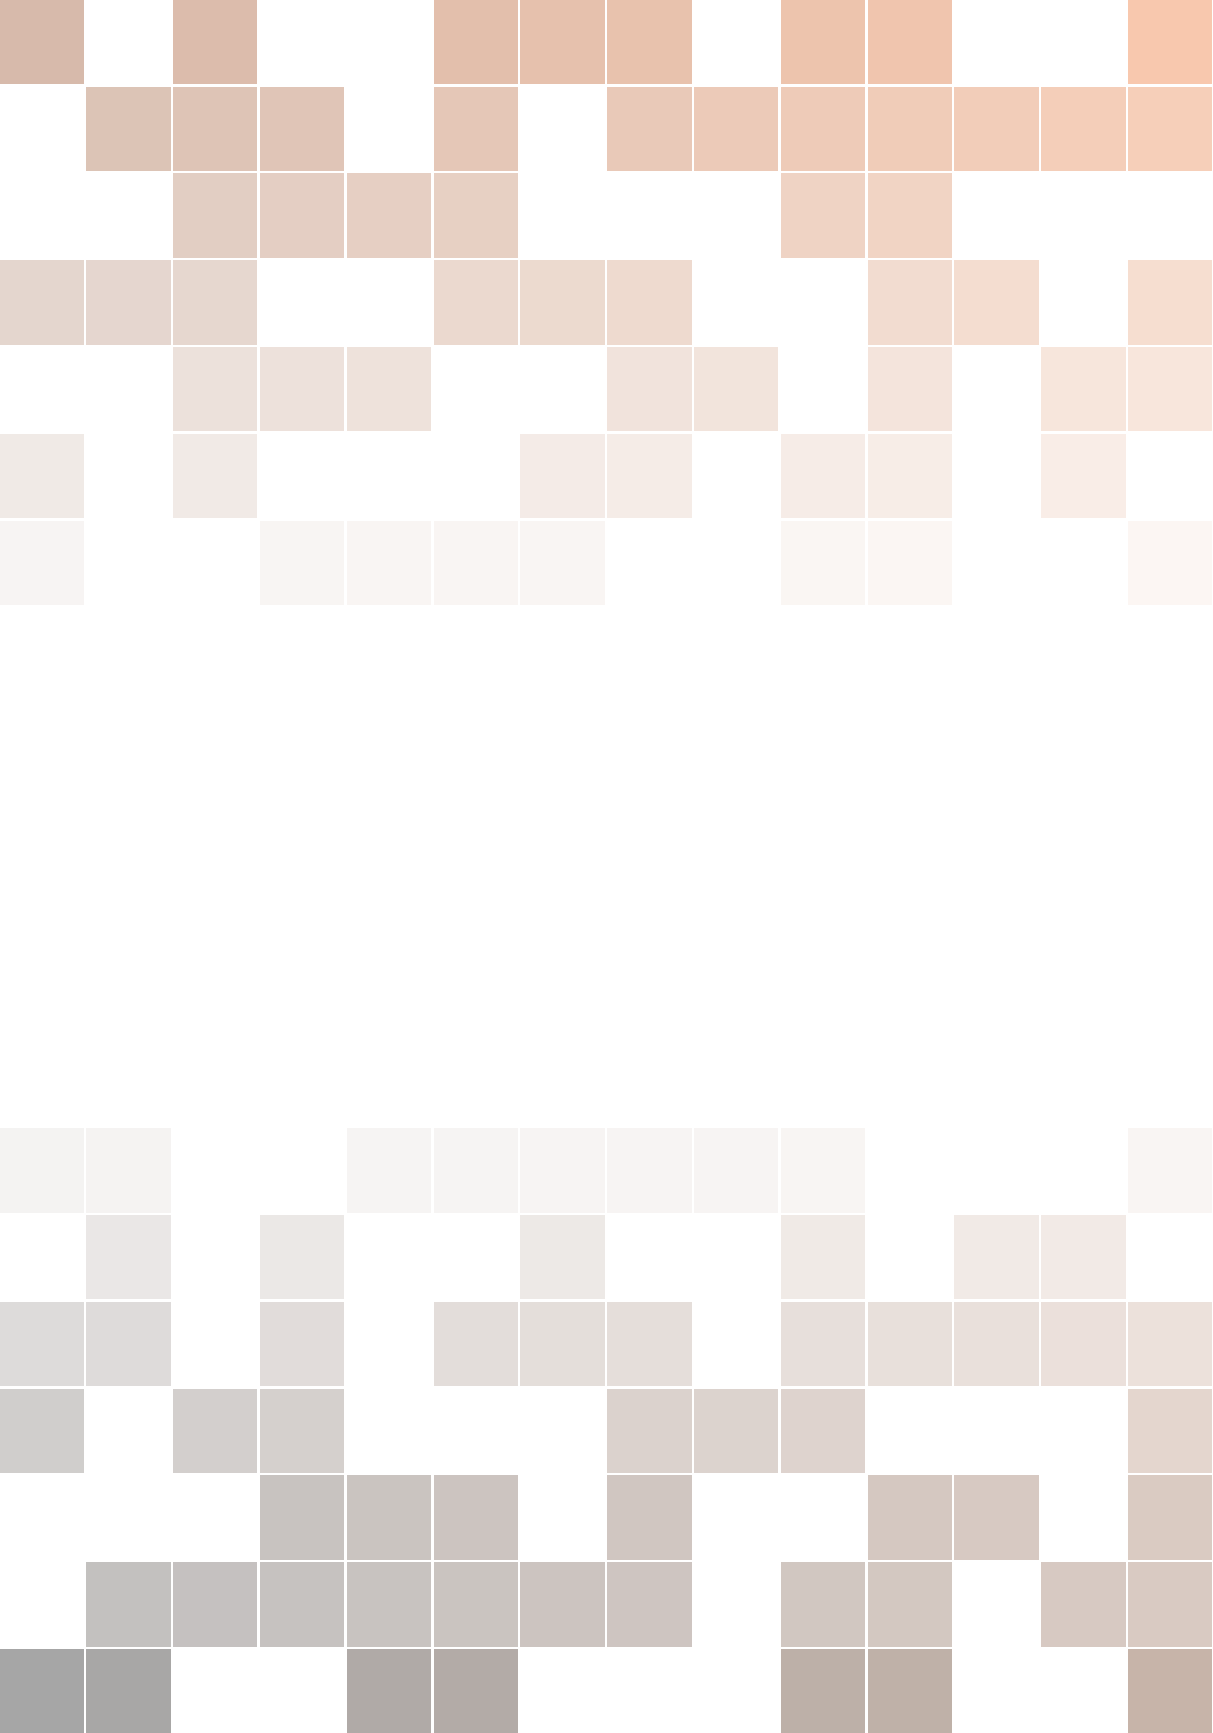
\includegraphics[scale=1]{background_main}}} % Image background
\centering
\vspace*{9.35cm}
\par\normalfont\fontsize{29}{30}\sffamily\selectfont
The \fmipp \matlab Toolbox for Windows\par % Book title
\vspace*{0.5cm}
{\huge Documentation}\\[5pt]
{\normalsize v\yyyymmdddate\today\versionsep\currenttime}\par % Subtitle
\endgroup

%----------------------------------------------------------------------------------------
%	COPYRIGHT PAGE
%----------------------------------------------------------------------------------------

\newpage
~\vfill
\thispagestyle{empty}


\noindent \matlab~\textregistered~is a registered trademark of The MathWorks, Inc.

\noindent Other product or brand names are trademarks or registered trademarks of their respective holders.

\vspace*{2cm}

\noindent Copyright \copyright\ 2016 AIT Austrian Institute of Technology\\ % Copyright notice

%\noindent \textsc{Published by Publisher}\\ % Publisher

\noindent Available at: \url{http://matlab-fmu.sourceforge.net/}\\ % URL

\noindent Licensed under the Creative Commons Attribution-NonCommercial 3.0 Unported License (the ``License''). You may not use this file except in compliance with the License. You may obtain a copy of the License at \url{http://creativecommons.org/licenses/by-nc/3.0}. Unless required by applicable law or agreed to in writing, software distributed under the License is distributed on an \textsc{``as is'' basis, without warranties or conditions of any kind}, either express or implied. See the License for the specific language governing permissions and limitations under the License.\\ % License information

%\noindent \textit{First printing, March 2013} % Printing/edition date

%----------------------------------------------------------------------------------------
%	TABLE OF CONTENTS
%----------------------------------------------------------------------------------------

\chapterimage{toc_head.pdf} % Table of contents heading image

\pagestyle{empty} % No headers

\tableofcontents % Print the table of contents itself

%\cleardoublepage % Forces the first chapter to start on an odd page so it's on the right

\pagestyle{fancy} % Print headers again

%----------------------------------------------------------------------------------------
%	CHAPTERS
%----------------------------------------------------------------------------------------

\chapterimage{chapter_head.pdf} % Chapter heading image

\chapter{Introduction}


\section{About}


\section{Basic functionality}

\chapter{Installation and Configuration}

\section{Software requirements}

The \fmipp \matlab FMU Export Utility is intended to run on Windows~7~(32-bit).
A working \matlab installation is required.
The toolbox has been tested with \matlab~R2013a.


When exporting \matlab functionality as an FMU for Co-Simulation, a working \matlab installation is also required on the system where the FMU is used (with a valid license for all the \matlab toolboxes that are used by the FMU).
Furthermore, for the export of FMUs the following tools need to be installed:
\begin{itemize}

  \item \href{https://www.microsoft.com/en-us/download/details.aspx?id=44914}{Microsoft Visual Studio Express 2013}

  \item \href{https://www.python.org/}{Python~2}
  
\end{itemize}


\section{Installation}
\label{sec:install}

To install the \fmipp \matlab Toolbox proceed as follows:
\begin{itemize}
  \item Download the latest version of the toolbox as ZIP-file from the \href{https://sourceforge.net/projects/matlab-fmu/files/latest/download}{download page}.
  
  \item Unzip the installation file into any sub directory (referred to as the \emph{installation folder}).
  
  \item Create a new Windows environment variable called \texttt{MATLAB\_FMIPP\_ROOT} that points to the installation folder.
  See for instance \href{http://www.computerhope.com/issues/ch000549.htm}{here} for instructions how to do that.
\end{itemize}


\section{Setting the \matlab path}

Whenever starting \matlab, run the script \texttt{setup.m} in the installation folder to use the \fmipp \matlab toolbox:
\begin{verbatim}
  >> cd( getenv( 'MATLAB_FMIPP_ROOT' ) )
  >> setup
\end{verbatim}
Alternatively, you can use the following two lines in any \matlab script to load the toolbox:
\begin{verbatim}
  fmippPath = getenv( 'MATLAB_FMIPP_ROOT' );
  addpath( genpath( fullfile( fmippPath, 'packages' ) ) );
\end{verbatim}


\section{Example}

For instance, after unzipping the toolbox to \texttt{C:{\textbackslash}Program~Files{\textbackslash}matlab-fmipp}, specify this path as the value of environment variable \texttt{MATLAB\_FMIPP\_ROOT}.
To use the toolbox, start \matlab and change to the installation folder:
\begin{verbatim}
  >> cd 'C:\Program Files\matlab-fmipp'
\end{verbatim}
Then run the setup script by typing:
\begin{verbatim}
  >> setup
\end{verbatim}

\chapter{Importing FMUs into \matlab}


\section{About}

The \href{https://fmi-standard.org/}{Functional Mock-up Interface}~(FMI) specification intentionally provides only the most essential and fundamental functionalities in the form of a C interface.
On the one hand, this increases flexibility in use and portability to virtually any platform.
On the other hand, such a low-level approach implies several prerequisites a simulation tool has to fulfil in order to be able to utilize such an FMI component.

The \fmipp \matlab Toolbox provides a wrapper for the \href{http://fmipp.sourceforge.net}{\fmipp Library}, which intends to bridge the gap between the basic functionality provided by the FMI specification and the typical requirements of simulation tools.
The \fmipp Library provides high-level functionality that eases the handling and manipulation of FMUs, such as numerical integration, advanced event-handling or state predictions.
This allows FMUs to be used more easily, e.g., integrating it into fixed time step or discrete event simulations.

This toolbox provides a stand-alone version of the \matlab interface for the \href{http://fmipp.sourceforge.net}{\fmipp Library} for Windows.
For other operating systems, this package can be built from \href{http://sourceforge.net/p/fmipp/code/ci/master/tree/}{source}.


\section{Example Usage}

The \emph{fmippim} package provides classes that allow to manipulate FMUs for ModelExchange and for Co-Simulation.
In the following, short descriptions and code snippets of the provided functionality demonstrate their usage.
More extensive background information can be found in the documentation of the \href{http://fmipp.sourceforge.net}{\fmipp Library}


\subsection{Loading the library}

FMUs are basically ZIP archives.
Before they can be used, they have to be extracted (unzipped), for instance with the help of \matlab's \texttt{unzip} function.
To load the library type:

\begin{verbatim}
  fmippPath = getenv( 'MATLAB_FMIPP_ROOT' );
  addpath( genpath( fullfile( fmippPath, 'packages' ) ) );
\end{verbatim}

\subsection{Classes FMUModelExchangeV1 and FMUModelExchangeV2}

The most obvious obstacle for using a bare FMU for ModelExchange is its lack of an integrator.
For this reason, classes \texttt{FMUModelExchangeV1} and \texttt{FMUModelExchangeV2} provide generic methods for the integration of FMUs for ModelExchange for FMI Version 1.0 and 2.0, respectively.
Instances of these classes own the actual FMU instance and are able to advance the current state up to a specified point in time, including the
proper handling of FMU-internal events.
The classes also provide functionality for convenient input and output handling.

The following example demonstrates the basic usage of class \texttt{FMUModelExchangeV1} (usage of class \texttt{FMUModelExchangeV2} is analogous).

First, specify the FMU's model name and the path to the unzipped FMU (as URI):
\begin{verbatim}
model_name = 'StandaloneRadiator';
uri_to_extracted_fmu = 'file:///C:/path/to/unzipped/StandaloneRadiator';
\end{verbatim}
Then, specify the FMU's configuration parameters and load the FMU:
\begin{verbatim}
logging_on = fmippim.fmiTrue();
stop_before_event = fmippim.fmiTrue();
event_search_precision = 1e-2;
integrator_type = fmippim.bdf(); % CVODE solver (Backward Differentiation Formula).

fmu = fmippim.FMUModelExchangeV1( uri_to_extracted_fmu,
                                  model_name,
                                  logging_on,
                                  stop_before_event,
                                  event_search_precision,
                                  integrator_type )
\end{verbatim}
Instantiate the FMU:
\begin{verbatim}
status = fmu.instantiate( 'standalone_radiator1' )
if status ~= fmippim.fmiOK(); error( 'instantiation not successful' ); end
\end{verbatim}
Set value of parameters:
\begin{verbatim}
Tlow = 82.0;
status = fmu.setRealValue( 'Tlow', Tlow )
if status ~= fmippim.fmiOK(); error( 'setRealValue not successful' ); end
\end{verbatim}
Initialize the FMU.
\begin{verbatim}
status = fmu.initialize()
if status ~= fmippim.fmiOK(); error( 'initialzation not successful' ); end
\end{verbatim}
Specify default step size of one integration step and the internal integrator step size, then start the simulation loop. The integrator always tries to make a full step, but it stops in case an event is detected.
\begin{verbatim}
stepsize = 300;
integrator_stepsize = stepsize/10;

t = 0;
tstop = 4 * 60 * 60;

while t < tstop
    t = fmu.integrate( t + stepsize, integrator_stepsize );

    T = fmu.getRealValue( 'T' );
    derT = fmu.getRealValue( 'derT' );

    if ( ( abs( T - Thigh ) < 1e-2 ) && ( derT > 0 ) )
        fmu.setRealValue( 'Pheat', 0.0 );  % turn off heating
    elseif ( ( abs( T - Tlow ) < 1e-2 ) && ( derT < 0 ) )
        fmu.setRealValue( 'Pheat', 1e3 );  % turn on heating
    end
end
\end{verbatim}
	
The integration algorithms provided by ODEINT and SUNDIALS can be chosen with an appropriate flag in the constructor (see example above).
The following algorithms are available:

\begin{center}

\begin{tabular}{|l|l|l|l|l|}
\hline 
Stepper & Name & Suite & Order & Adaptive \\ 
\hline 
eu & Explicit Euler & ODEINT & 1 & No  \\ 
\hline 
rk & 4th order Runge-Kutta & ODEINT & 4 & No  \\ 
\hline 
abm & Adams-Bashforth-Moulton & ODEINT & 8 & No  \\ 
\hline 
ck & Cash-Karp & ODEINT & 5 & Yes  \\ 
\hline 
dp & Dormand-Prince & ODEINT & 5 & Yes  \\ 
\hline 
fe & Fehlberg & ODEINT & 8 & Yes  \\ 
\hline 
bs & Bulirsch Stoer & ODEINT & 1-16 & Yes  \\ 
\hline 
ro & Rosenbrock & ODEINT & 4 & Yes  \\ 
\hline 
bdf & Backward Differentiation Formula & SUNDIALS & 1-5 & Yes  \\ 
\hline 
abm2 & Adams-Bashforth-Moulton & SUNDIALS & 1-12 & Yes \\ 
\hline 
\end{tabular} 

\end{center}

\chapter{Exporting \matlab scripts as FMUs}

\section{Class FMIAdapter}

The functionality of \matlab can be made available as FMU for Co-Simulation (version 1.0) with the help of class \texttt{FMIAdapter} (contained in package \texttt{fmipputils}).
This class defines two abstract methods that have to be implemented by the user:
\begin{itemize}

  \item Method \texttt{init( obj, currentCommunicationPoint )} is intended to initialize input/output variables and parameters needed for co-simulation.
  Optionally, a fixed simulation time step can be specified.

  \item Method \texttt{doStep(  obj, currentCommunicationPoint, communicationStepSize )} is called at every simulation step (as requested by the master algorithm).
\end{itemize}
By deriving a new class from \texttt{class FMIAdapter} and implementing these two methods, virtually all functionality of \matlab can be made available via an FMU for Co-Simulation.
When using such an FMU, \matlab is started in the background and synchronized to the master algorithm.

For initializing input/output variables and parameters of type \texttt{fmiReal}, class \texttt{FMIAdapter} provides the following methods:
\begin{itemize}
  \item \texttt{function defineRealParameters( obj, parameterNames )}
  \item \texttt{function defineRealInputs( obj, inputVariableNames )}
  \item \texttt{function defineRealOutputs( obj, outputVariableNames )}
\end{itemize}
Their input arguments are cell arrays containing the corresponding names as string.
For initializing input/output variables and parameters of other types (\texttt{fmiInteger}, \texttt{fmiBoolean}, \texttt{fmiString}) corresponding functions are available.

Fixed time step simulation can be enforced by calling the following method:
\begin{itemize}
  \item \texttt{function enforceTimeStep( obj, stepSize )}
\end{itemize}

For getting the values of parameters and input variables as well as setting the values  of output variables of type \texttt{fmiReal}, class \texttt{FMIAdapter} provides another set of methods:
\begin{itemize}
  \item \texttt{function realParameterValues = getRealParameterValues( obj )}
  \item \texttt{function realInputValues = getRealInputValues( obj )}
  \item \texttt{function setRealOutputValues( obj, realOutputValues )}
\end{itemize}
The order in which values are retrieved or set corresponds to the order in which they were defined (see methods above).
For retrieving or setting input/output variables and parameters of other types (\texttt{fmiInteger}, \texttt{fmiBoolean}, \texttt{fmiString}) corresponding functions are available.

For instance, when defining two input variables called \texttt{X} and \texttt{Y}, the following function call has to be issued in the \texttt{init} method:
\begin{verbatim}
  obj.defineRealInputs( { "X", "Y" } );
\end{verbatim}
In the \texttt{doStep} methods, the values corresponding to these input variables can be retrieved like this:
\begin{verbatim}
  [ x, y ] = obj.getRealInputValues();
\end{verbatim}


\section{Creating an FMU}

Creating an FMU from a class inherited from \texttt{FMIAdapter} can be done by calling function \texttt{createFMU}:
\begin{itemize}
  \item \texttt{function createFMU( modelID, classFileName, extra, useJVM )}
  \begin{itemize}
    \item \texttt{modelID} (string): Specifies the FMU's model identifier.
    \item \texttt{classFileName} (string): Specifies the path to the file containing the class definition.
    \item \texttt{extra} (string): Specifies additional files (data files, \matlab scripts, etc.) that should be added to the FMU.
    \item \texttt{useJVM} (boolean): This optional input argument specifies whether the Java Virtual Machine (\matlab GUI) should be started when using the FMU (default: \texttt{false}).
  \end{itemize}
\end{itemize}
\chapter{Example}

\section{Overview}

\section{\matlab script}

\section{Creating the FMU}

\section{Using the FMU}

\subsection{Results}

\chapter{Troubleshooting}


\chapter{Appendix}

\section{The \fmipp \matlab Toolbox License}
\label{matlab_fmu_license}

Copyright (c) 2019, AIT Austrian Institute of Technology GmbH. All
rights reserved.

Redistribution and use in source and binary forms, with or without
modification, are permitted provided that the following conditions are
met:

\begin{itemize}
\itemsep1pt\parskip0pt\parsep0pt
\item
  Redistributions of source code must retain the above copyright notice,
  this list of conditions and the following disclaimer.
\item
  Redistributions in binary form must reproduce the above copyright
  notice, this list of conditions and the following disclaimer in the
  documentation and/or other materials provided with the distribution.
\end{itemize}

THIS SOFTWARE IS PROVIDED BY THE COPYRIGHT HOLDERS AND CONTRIBUTORS ``AS
IS'' AND ANY EXPRESS OR IMPLIED WARRANTIES, INCLUDING, BUT NOT LIMITED
TO, THE IMPLIED WARRANTIES OF MERCHANTABILITY AND FITNESS FOR A
PARTICULAR PURPOSE ARE DISCLAIMED. IN NO EVENT SHALL THE COPYRIGHT
HOLDER OR CONTRIBUTORS BE LIABLE FOR ANY DIRECT, INDIRECT, INCIDENTAL,
SPECIAL, EXEMPLARY, OR CONSEQUENTIAL DAMAGES (INCLUDING, BUT NOT LIMITED
TO, PROCUREMENT OF SUBSTITUTE GOODS OR SERVICES; LOSS OF USE, DATA, OR
PROFITS; OR BUSINESS INTERRUPTION) HOWEVER CAUSED AND ON ANY THEORY OF
LIABILITY, WHETHER IN CONTRACT, STRICT LIABILITY, OR TORT (INCLUDING
NEGLIGENCE OR OTHERWISE) ARISING IN ANY WAY OUT OF THE USE OF THIS
SOFTWARE, EVEN IF ADVISED OF THE POSSIBILITY OF SUCH DAMAGE.


\section{The \fmipp License}
\label{fmipp_license}

Copyright (c) 2018, AIT Austrian Institute of Technology GmbH. All
rights reserved.

Redistribution and use in source and binary forms, with or without
modification, are permitted provided that the following conditions are
met:

\begin{itemize}
\itemsep1pt\parskip0pt\parsep0pt
\item
  Redistributions of source code must retain the above copyright notice,
  this list of conditions and the following disclaimer.
\item
  Redistributions in binary form must reproduce the above copyright
  notice, this list of conditions and the following disclaimer in the
  documentation and/or other materials provided with the distribution.
\end{itemize}

THIS SOFTWARE IS PROVIDED BY THE COPYRIGHT HOLDERS AND CONTRIBUTORS ``AS
IS'' AND ANY EXPRESS OR IMPLIED WARRANTIES, INCLUDING, BUT NOT LIMITED
TO, THE IMPLIED WARRANTIES OF MERCHANTABILITY AND FITNESS FOR A
PARTICULAR PURPOSE ARE DISCLAIMED. IN NO EVENT SHALL THE COPYRIGHT
HOLDER OR CONTRIBUTORS BE LIABLE FOR ANY DIRECT, INDIRECT, INCIDENTAL,
SPECIAL, EXEMPLARY, OR CONSEQUENTIAL DAMAGES (INCLUDING, BUT NOT LIMITED
TO, PROCUREMENT OF SUBSTITUTE GOODS OR SERVICES; LOSS OF USE, DATA, OR
PROFITS; OR BUSINESS INTERRUPTION) HOWEVER CAUSED AND ON ANY THEORY OF
LIABILITY, WHETHER IN CONTRACT, STRICT LIABILITY, OR TORT (INCLUDING
NEGLIGENCE OR OTHERWISE) ARISING IN ANY WAY OUT OF THE USE OF THIS
SOFTWARE, EVEN IF ADVISED OF THE POSSIBILITY OF SUCH DAMAGE.

\section{The \boost Software License}
\label{boost_license}

Version 1.0 - August 17th, 2003

Permission is hereby granted, free of charge, to any person or organization
obtaining a copy of the software and accompanying documentation covered by
this license (the "Software") to use, reproduce, display, distribute,
execute, and transmit the Software, and to prepare derivative works of the
Software, and to permit third-parties to whom the Software is furnished to
do so, all subject to the following:

The copyright notices in the Software and this entire statement, including
the above license grant, this restriction and the following disclaimer,
must be included in all copies of the Software, in whole or in part, and
all derivative works of the Software, unless such copies or derivative
works are solely in the form of machine-executable object code generated by
a source language processor.

THE SOFTWARE IS PROVIDED "AS IS", WITHOUT WARRANTY OF ANY KIND, EXPRESS OR
IMPLIED, INCLUDING BUT NOT LIMITED TO THE WARRANTIES OF MERCHANTABILITY,
FITNESS FOR A PARTICULAR PURPOSE, TITLE AND NON-INFRINGEMENT. IN NO EVENT
SHALL THE COPYRIGHT HOLDERS OR ANYONE DISTRIBUTING THE SOFTWARE BE LIABLE
FOR ANY DAMAGES OR OTHER LIABILITY, WHETHER IN CONTRACT, TORT OR OTHERWISE,
ARISING FROM, OUT OF OR IN CONNECTION WITH THE SOFTWARE OR THE USE OR OTHER
DEALINGS IN THE SOFTWARE.

\section{Version History}

\begin{itemize}
  \item v0.1: first release version
  \item v0.2: added support for importing FMU for Co-Simulation v2.0, addded support for Python 3
  \item v0.3: switched to 64-bit
\end{itemize}



%----------------------------------------------------------------------------------------
%	INDEX
%----------------------------------------------------------------------------------------

%\cleardoublepage
%\phantomsection
%\setlength{\columnsep}{0.75cm}
%\addcontentsline{toc}{chapter}{\textcolor{ocre}{Index}}
%\printindex

%----------------------------------------------------------------------------------------

\end{document}
